\begin{frame}
    \frametitle{\textcolor{blue}{TX}/\textcolor{red}{RX} Placement}
    \begin{columns}
        \begin{column}[t]{0.33\textwidth}
            \begin{center}
                \textbf{Monostatic}
                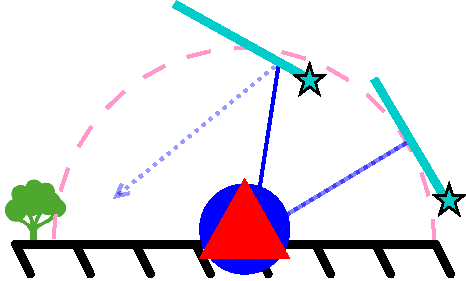
\includegraphics[height=2cm]{img/monostatic_scatter.pdf}
            \end{center}
            Co-located \textcolor{blue}{\textbf{TX}} and \textcolor{red}{\textbf{RX}}
            \begin{itemize}
                \footnotesize
                \item[\checkmark] Simple
                \item[\checkmark] Commercially available 
                \item[\(\times\)] Limited capabilities 
            \end{itemize}
        \end{column}
        \begin{column}[t]{0.33\textwidth}
            \uncover<2->{\begin{center}
                \textbf{Bistatic}
                \uncovergraphics<2->[height=2cm]{img/bistatic_scatter.pdf}
            \end{center}
            Separated \textcolor{blue}{\textbf{TX}} and \textcolor{red}{\textbf{RX}}
            \begin{itemize}
                \footnotesize
                \item[\checkmark] Enables new techniques
                \item[\checkmark] Supports different geometric diversity
                \item[\(\blacktriangleright\)] Requires time synchronization 
            \end{itemize}}
        \end{column}
        \begin{column}[t]{0.33\textwidth}
            \uncover<3->{\begin{center}
                \textbf{Multistatic}
                \uncovergraphics<3->[height=2cm]{img/multistatic_network.pdf}
            \end{center}
            Network of many \textcolor{blue}{\textbf{TX}} and \textcolor{red}{\textbf{RX}}
            \begin{itemize}
                \footnotesize
                \item[\checkmark] Widest coverage
                \item[\checkmark] Increased geometric diversity and counts
                \item[\checkmark] Incrementally expandable
                \item[\(\blacktriangleright\)] Increased complexity  
            \end{itemize}}
        \end{column}
    \end{columns}
\end{frame}
